\documentclass[a4paper]{article}
\usepackage[a4paper,margin=0mm]{geometry}
\usepackage{fontspec}
\usepackage{unicode-math}
\usepackage{tikz}
\usetikzlibrary{calc}
\usepackage[table]{xcolor}
\usepackage[absolute]{textpos}
\usepackage{enumitem}
\usepackage{array}
\usepackage{multirow}

\setmainfont{Libertinus Serif}
\setsansfont{Libertinus Sans}
\setmathfont{Libertinus Math}

\definecolor{accent}{HTML}{0F6A52}
\definecolor{badge}{HTML}{A9CFC2}
\definecolor{ink}{HTML}{2A2E30}

\setlength{\TPHorizModule}{1mm}
\setlength{\TPVertModule}{1mm}
\setlength{\parindent}{0pt}
\pagestyle{empty}
\binoppenalty=10000 \relpenalty=10000

\newcommand{\LCOL}{16mm}
\newcommand{\RCOL}{111mm}
\newcommand{\COLW}{83mm}

\newcommand{\topicheader}[2]{%
\begin{textblock*}{194mm}(16mm,10mm)
\begin{tikzpicture}
\node[fill=accent,text=white,font=\sffamily\bfseries\fontsize{13}{13}\selectfont,
      minimum width=9mm,minimum height=9mm,inner sep=0pt] at (4.5mm,-4.5mm) {#1};
\node[font=\sffamily\bfseries\fontsize{15}{16}\selectfont,text=ink,anchor=west] at (12mm,-4.5mm) {#2};
\end{tikzpicture}
\end{textblock*}
\begin{textblock*}{194mm}(16mm,22.5mm)

\begin{tikzpicture}
\fill[accent] (0,0) rectangle (194mm,0.5mm);
\end{tikzpicture}
\end{textblock*}
}

\newcommand{\pagefooter}[1]{%
\begin{textblock*}{194mm}(8mm,286.41mm)
  
\begin{tikzpicture}
    \fill[accent] (0,0) rectangle (194mm,0.6mm);
  \end{tikzpicture}
\end{textblock*}
\begin{textblock*}{63.59mm}(8mm,288.27mm)
  {\sffamily\bfseries\color{accent}\fontsize{13}{16}\selectfont SAT 1200+}
\end{textblock*}
\begin{textblock*}{10mm}(188mm,288.27mm)
  \centering{\sffamily\color{accent}\fontsize{14}{16}\selectfont #1}
\end{textblock*}
}

\newcommand{\colrule}[2]{%
\begin{textblock*}{1mm}(105mm,#1mm)
\begin{tikzpicture}
\draw[black!65,line width=0.5pt] (0,0) -- (0,#2mm);
\end{tikzpicture}
\end{textblock*}
}

% Page kicker: left = module line, right = question range
\newcommand{\pagekicker}[2]{%
\begin{textblock*}{194mm}(16mm,25.2mm)
{\sffamily\bfseries\fontsize{10.5}{12}\selectfont\color{accent}#1}\hfill{\sffamily\fontsize{10}{12}\selectfont\color{black!70}#2}
\end{textblock*}
}

\setlength{\fboxsep}{1.4pt}
\setlength{\fboxrule}{0.5pt}
\newcommand{\pnum}[1]{\fcolorbox{ink}{white}{\sffamily\bfseries\fontsize{8}{8}\selectfont #1}~}

% centered display line inside a stem
\newcommand{\dsp}[1]{\par\vspace{1.4mm}\centerline{#1}\vspace{1.8mm}}

% student-produced response box
\newcommand{\gridbox}{%
\par\vspace{3mm}\noindent

\begin{tikzpicture}
\node[anchor=south west,font=\sffamily\bfseries\fontsize{7.5}{9}\selectfont,text=accent,inner sep=0pt] at (0,0.3mm) {STUDENT-PRODUCED RESPONSE};
\draw[ink,line width=0.7pt] (0,-9.5mm) rectangle (40mm,-0.8mm);
\node[anchor=west,font=\sffamily\fontsize{7.5}{9}\selectfont,text=black!55,inner sep=0pt] at (43mm,-5.2mm) {Write your answer in the box.};
\end{tikzpicture}\par}

\arrayrulecolor{accent}
\setlength{\arrayrulewidth}{0.7pt}
\renewcommand{\arraystretch}{1.35}

\newcommand{\figwrap}[1]{\par\vspace{2.5mm}\centerline{{\arrayrulecolor{ink}\setlength{\arrayrulewidth}{0.5pt}\renewcommand{\arraystretch}{1.3}#1}}\vspace{0.5mm}}

\begin{document}

% ================= PAGE 1: Mock Test 7 -- instructions + geometry reference sheet =================
\topicheader{7}{Mock Test 7}
\pagefooter{1}
\mbox{}%

\newcommand{\cardhead}[1]{{\sffamily\bfseries\color{accent}\fontsize{11.5}{14}\selectfont #1}\par\vspace{0.6mm}%
{\color{accent}\rule{\linewidth}{0.5pt}}\par\vspace{1.6mm}}
\newcommand{\bul}{\item[\textcolor{accent}{\rule[0.2mm]{1.5mm}{1.5mm}}]}

\begin{textblock*}{194mm}(16mm,28mm)
{\sffamily\bfseries\color{accent}\fontsize{26}{28}\selectfont Mock Test 7\par}
\vspace{1mm}
{\sffamily\color{ink}\fontsize{11}{14}\selectfont Full-length digital SAT Math practice \;\textperiodcentered\; 2 modules $\times$ 22 questions $\times$ 35 minutes\par}
\end{textblock*}

\begin{textblock*}{\COLW}(\LCOL,53mm)
{\fontsize{9.4}{12.2}\selectfont
\cardhead{How this test works}
\renewcommand{\arraystretch}{1.3}\setlength{\tabcolsep}{4pt}
\noindent\begin{tabular}{|>{\raggedright\arraybackslash}p{20mm}|>{\centering\arraybackslash}p{15mm}|>{\centering\arraybackslash}p{13mm}|>{\centering\arraybackslash}p{19mm}|}
\hline
\rowcolor{badge!55}\textbf{Module} & \textbf{Questions} & \textbf{Time} & \textbf{Calculator}\\\hline
Module 1 & 22 & 35 min & allowed\\\hline
Module 2 & 22 & 35 min & allowed\\\hline
\end{tabular}\par\vspace{2.2mm}
\begin{itemize}[leftmargin=5mm,itemsep=1.2mm,topsep=0mm,parsep=0mm]
\bul Time each module separately: 35 minutes, not a minute more. Rest for 5--10 minutes between the two modules.
\bul Use a calculator (the built-in Desmos graphing calculator or any approved calculator) on both modules.
\bul Module 1 is a standard mix of easy, medium and hard questions. Module 2 is the \emph{harder route} you reach by doing well on Module 1.
\bul Answer every question. There is no penalty for a wrong answer.
\bul Unless a problem says otherwise, all numbers are real, a function's domain is every real number for which it is defined, and figures are not necessarily drawn to scale.
\bul Do not look at any answers while you work. When you finish both modules, score yourself with the \textbf{Answer Sheets} section at the end of this book.
\end{itemize}
}
\end{textblock*}

\begin{textblock*}{\COLW}(\RCOL,53mm)
{\fontsize{9.4}{12.2}\selectfont
\cardhead{Student-produced responses (grid-ins)}
Some questions have no answer choices. Work out the answer and write it in the answer box (on the real test you type it in).
\begin{itemize}[leftmargin=5mm,itemsep=1.2mm,topsep=1.6mm,parsep=0mm]
\bul You may give an integer, a decimal, or a fraction. For one answer, $9/2$ and $4.5$ are both correct.
\bul Never enter a mixed number: write $7/2$ or $3.5$, not $3\,1/2$ (it would be read as $31/2$).
\bul Do not enter symbols or units such as \$, \%, or $\pi$. Enter the number only.
\bul An answer may use at most 5 characters (6 if it is negative), counting the slash and the decimal point.
\bul If an answer is a repeating decimal, enter it as a fraction such as $2/3$, or fill all the digits that fit: $0.6666$ or $0.6667$.
\bul If you find more than one correct answer, enter only one of them.
\end{itemize}
\vspace{1.2mm}
\noindent\fcolorbox{accent}{badge!25}{\parbox{\dimexpr\linewidth-2\fboxsep-2\fboxrule}{\centering\sffamily\fontsize{8.5}{11}\selectfont
\textbf{Example.} Answer $4\tfrac12$ \;$\rightarrow$\; enter \textbf{9/2} or \textbf{4.5}\par}}
\par\vspace{3mm}
\noindent{\sffamily\bfseries\color{accent}Pacing.}\ Q1--15: about 18 min. Q16--22: about 17 min. Keep the last 2--3 min for flagged questions and every blank grid-in (a blank is a guaranteed zero).
}
\end{textblock*}

% ---- Geometry reference sheet (full width card) ----
\begin{textblock*}{178mm}(16mm,156mm)
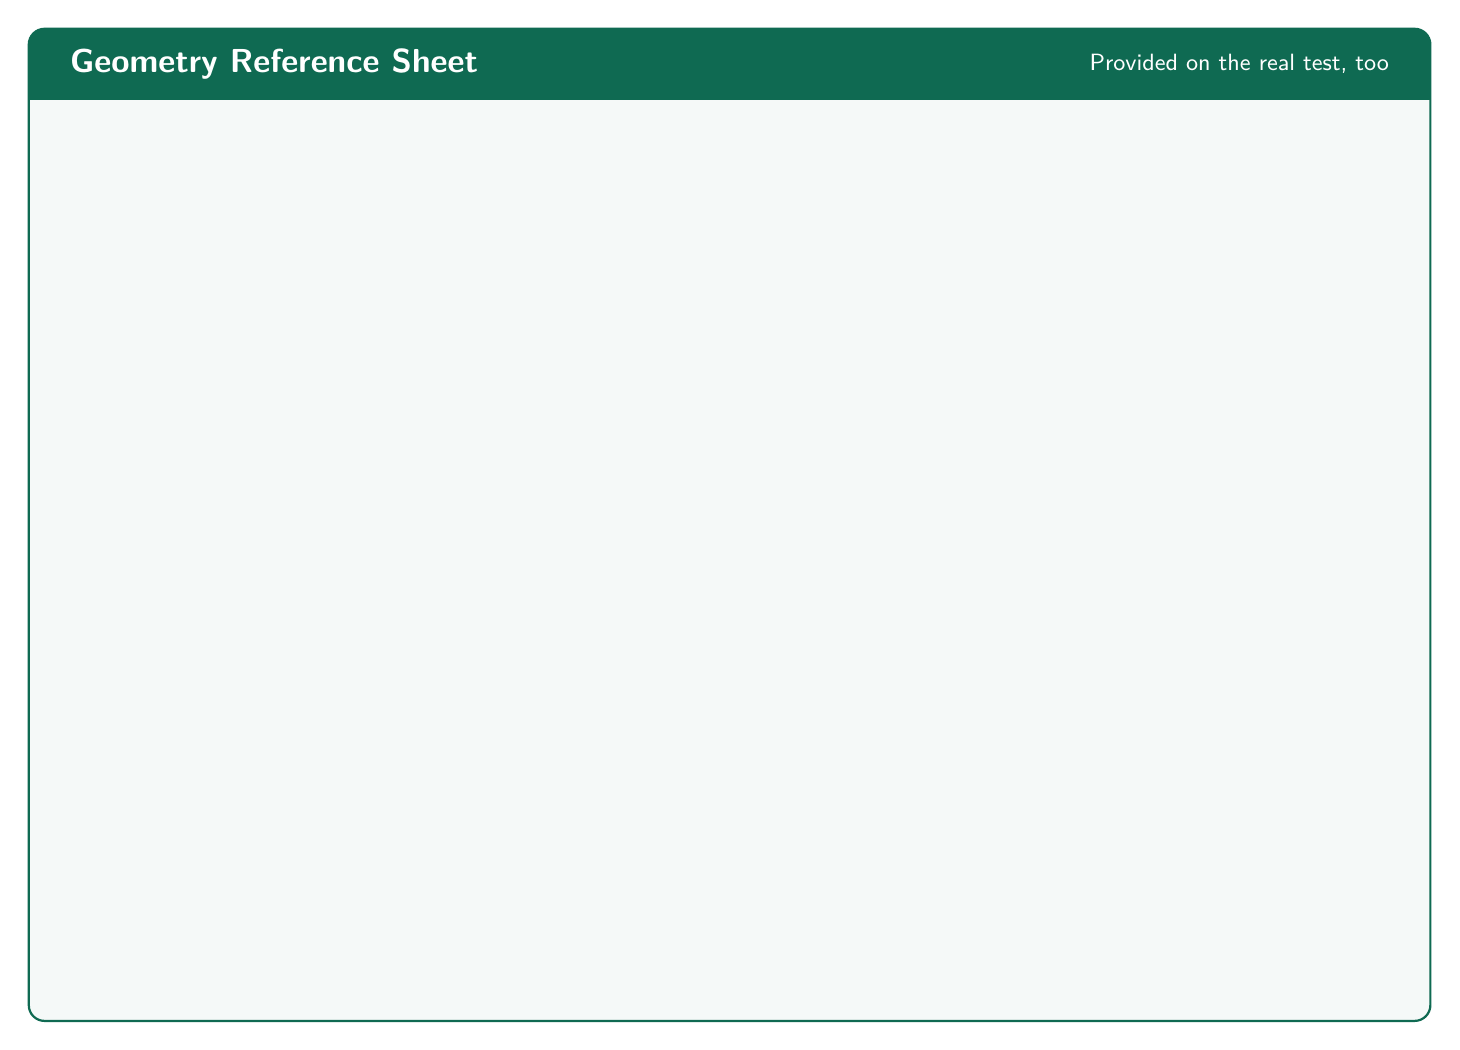
\begin{tikzpicture}
\draw[accent,line width=0.8pt,rounded corners=2mm,fill=badge!12] (0,0) rectangle (178mm,-126mm);
\fill[accent,rounded corners=2mm] (0,0) rectangle (178mm,-9mm);
\fill[accent] (0,-5mm) rectangle (178mm,-9mm);
\node[anchor=west,text=white,font=\sffamily\bfseries\fontsize{12}{14}\selectfont] at (4mm,-4.5mm) {Geometry Reference Sheet};
\node[anchor=east,text=white,font=\sffamily\fontsize{8.5}{10}\selectfont] at (174mm,-4.5mm) {Provided on the real test, too};
\end{tikzpicture}
\end{textblock*}

\newcommand{\refcell}[3]{\begin{textblock*}{42mm}(#1mm,#2mm)\begin{minipage}[t][36mm][t]{42mm}\centering #3\end{minipage}\end{textblock*}}
\newcommand{\refin}[2]{\parbox[b][26mm][b]{42mm}{\centering #1}\par\vspace{1.6mm}{\fontsize{9.6}{11.5}\selectfont #2}}
\tikzset{rf/.style={ink,line width=0.65pt},lb/.style={font=\fontsize{8.5}{9.5}\selectfont,inner sep=1.2pt}}

% ---------- row 1
\refcell{18}{167}{\refin{\begin{tikzpicture}[scale=1.25]
\draw[rf] (0,0) circle (9mm); \draw[rf] (0,0)--(9mm,0); \fill[ink] (0,0) circle (0.7pt);
\node[lb,above] at (4.5mm,0) {$r$};
\end{tikzpicture}}{Circle\\$A=\pi r^{2}$,\; $C=2\pi r$}}
\refcell{62}{167}{\refin{\begin{tikzpicture}[scale=1.25]
\draw[rf] (0,0) rectangle (22mm,12mm);
\node[lb,below] at (11mm,0) {$\ell$}; \node[lb,right] at (22mm,6mm) {$w$};
\end{tikzpicture}}{Rectangle\\$A=\ell w$}}
\refcell{106}{167}{\refin{\begin{tikzpicture}[scale=1.25]
\draw[rf] (0,0)--(22mm,0)--(7mm,13mm)--cycle;
\draw[rf,dashed] (7mm,0)--(7mm,13mm);
\draw[rf] (7mm,0)++(0,1.8mm)--++(1.8mm,0)--++(0,-1.8mm);
\node[lb,below] at (11mm,0) {$b$}; \node[lb,left] at (7mm,6.5mm) {$h$};
\end{tikzpicture}}{Triangle\\$A=\tfrac12 bh$}}
\refcell{150}{167}{\refin{\begin{tikzpicture}[scale=1.25]
\draw[rf] (0,0)--(18mm,0)--(0,12mm)--cycle;
\draw[rf] (0,1.8mm)--(1.8mm,1.8mm)--(1.8mm,0);
\node[lb,below] at (9mm,0) {$a$}; \node[lb,left] at (0,6mm) {$b$}; \node[lb,above right] at (9mm,6mm) {$c$};
\end{tikzpicture}}{Right triangle\\$c^{2}=a^{2}+b^{2}$}}

% ---------- row 2
\refcell{18}{204}{\refin{\begin{tikzpicture}[scale=1.25]
\draw[rf] (0,0)--(19.053mm,0)--(0,11mm)--cycle;
\draw[rf] (0,1.8mm)--(1.8mm,1.8mm)--(1.8mm,0);
\node[lb,below] at (9.5mm,0) {$x\sqrt3$}; \node[lb,left] at (0,5.5mm) {$x$}; \node[lb,above right] at (9.5mm,5.5mm) {$2x$};
\node[lb] at (14.6mm,1.9mm) {\fontsize{6.5}{7}\selectfont$30^\circ$}; \node[lb] at (3.2mm,8.2mm) {\fontsize{6.5}{7}\selectfont$60^\circ$};
\end{tikzpicture}}{$30^\circ$--$60^\circ$--$90^\circ$ triangle}}
\refcell{62}{204}{\refin{\begin{tikzpicture}[scale=1.25]
\draw[rf] (0,0)--(10mm,0)--(0,10mm)--cycle;
\draw[rf] (0,1.8mm)--(1.8mm,1.8mm)--(1.8mm,0);
\node[lb,below] at (5mm,0) {$s$}; \node[lb,left] at (0,5mm) {$s$}; \node[lb,above right] at (5mm,5mm) {$s\sqrt2$};
\end{tikzpicture}}{$45^\circ$--$45^\circ$--$90^\circ$ triangle}}
\refcell{106}{204}{\refin{\begin{tikzpicture}[scale=1.2]
\draw[rf] (0,0) rectangle (16mm,9mm);
\draw[rf] (16mm,9mm)--(22mm,13mm)--(6mm,13mm)--(0,9mm);
\draw[rf] (16mm,0)--(22mm,4mm)--(22mm,13mm);
\draw[rf,dashed] (6mm,13mm)--(6mm,4mm)--(22mm,4mm); \draw[rf,dashed] (0,0)--(6mm,4mm);
\node[lb,below] at (8mm,0) {$\ell$}; \node[lb,right] at (22mm,8.5mm) {$h$}; \node[lb,below right] at (19mm,2mm) {$w$};
\end{tikzpicture}}{Rectangular solid\\$V=\ell wh$}}
\refcell{150}{204}{\refin{\begin{tikzpicture}[scale=1.2]
\draw[rf] (0,2.2mm) ellipse (7mm and 2.2mm);
\draw[rf] (-7mm,2.2mm)--(-7mm,14mm); \draw[rf] (7mm,2.2mm)--(7mm,14mm);
\draw[rf] (0,14mm) ellipse (7mm and 2.2mm);
\draw[rf,dashed] (0,14mm)--(7mm,14mm); \fill[ink] (0,14mm) circle (0.6pt);
\node[lb,above] at (3.5mm,14mm) {$r$}; \node[lb,right] at (7mm,8mm) {$h$};
\end{tikzpicture}}{Right circular cylinder\\$V=\pi r^{2}h$}}

% ---------- row 3
\refcell{18}{241}{\refin{\begin{tikzpicture}[scale=1.15]
\draw[rf] (0,0) circle (10mm);
\draw[rf] (-10mm,0) arc (180:360:10mm and 2.8mm); \draw[rf,dashed] (-10mm,0) arc (180:0:10mm and 2.8mm);
\draw[rf] (0,0)--(10mm,0); \fill[ink] (0,0) circle (0.7pt); \node[lb,above] at (5mm,0) {$r$};
\end{tikzpicture}}{Sphere\\$V=\tfrac43\pi r^{3}$}}
\refcell{62}{241}{\refin{\begin{tikzpicture}[scale=1.2]
\draw[rf] (0,2.2mm) ellipse (7mm and 2.2mm);
\draw[rf] (-7mm,2.2mm)--(0,16mm)--(7mm,2.2mm);
\draw[rf,dashed] (0,16mm)--(0,2.2mm); \draw[rf,dashed] (0,2.2mm)--(7mm,2.2mm);
\fill[ink] (0,2.2mm) circle (0.6pt);
\node[lb,left] at (0,9.5mm) {$h$}; \node[lb,above] at (3.5mm,2.2mm) {$r$};
\end{tikzpicture}}{Right circular cone\\$V=\tfrac13\pi r^{2}h$}}
\refcell{106}{241}{\refin{\begin{tikzpicture}[scale=1.2]
\draw[rf] (0,0)--(16mm,0)--(22mm,4mm); \draw[rf] (0,0)--(10mm,15mm)--(16mm,0); \draw[rf] (10mm,15mm)--(22mm,4mm);
\draw[rf,dashed] (0,0)--(6mm,4mm)--(22mm,4mm); \draw[rf,dashed] (6mm,4mm)--(10mm,15mm);
\node[lb,below] at (8mm,0) {$\ell$}; \node[lb,below right] at (19mm,2mm) {$w$}; \node[lb,left] at (10mm,9.5mm) {$h$};
\end{tikzpicture}}{Rectangular pyramid\\$V=\tfrac13\ell wh$}}
\begin{textblock*}{40mm}(151mm,247mm)
{\fontsize{9.2}{12}\selectfont\raggedright
\textcolor{accent}{\rule[0.3mm]{1.6mm}{1.6mm}}\; A circle has 360 degrees of arc.\par\vspace{1.2mm}
\textcolor{accent}{\rule[0.3mm]{1.6mm}{1.6mm}}\; The angles of a triangle add up to 180 degrees.\par\vspace{1.2mm}
\textcolor{accent}{\rule[0.3mm]{1.6mm}{1.6mm}}\; $r$ radius, $\ell$ length, $w$ width, $b$ base, $h$ height.\par}
\end{textblock*}

\clearpage

% ===== Module 1, page 1 =====
\topicheader{7}{Mock Test 7}
\pagefooter{2}
\colrule{34}{236}
\mbox{}%
\pagekicker{Mock 7 \textperiodcentered{} Module 1 \textperiodcentered{} 22 questions \textperiodcentered{} 35 minutes}{Questions 1--8}
\begin{textblock*}{\COLW}(\LCOL,34mm)
{\fontsize{10.4}{13.4}\selectfont
\parbox[t][233mm][t]{\COLW}{%
\noindent\pnum{1} A diner charges \$8.50 for the lunch special plus \$1.25 for each extra topping. Ravi paid \$13.50 for a lunch special with extra toppings and nothing else. How many extra toppings did he order?\par\vspace{2.2mm}
\hspace*{7mm}(A)\ $5$\\[1.8mm]
\hspace*{7mm}(B)\ $10.8$\\[1.8mm]
\hspace*{7mm}(C)\ $4$\\[1.8mm]
\hspace*{7mm}(D)\ $17.6$
\vfill

\noindent\pnum{2} Which of the following is equivalent to $(2x+5)^2$?\par\vspace{2.2mm}
\hspace*{7mm}(A)\ $4x^2+20x+25$\\[1.8mm]
\hspace*{7mm}(B)\ $4x^2+25$\\[1.8mm]
\hspace*{7mm}(C)\ $4x^2+10x+25$\\[1.8mm]
\hspace*{7mm}(D)\ $2x^2+20x+25$
\vfill

\noindent\pnum{3} A restaurant sold 480 pizzas last week, and $\frac{3}{8}$ of them were pepperoni. How many of the pizzas sold were not pepperoni?\gridbox
\vfill

\noindent\pnum{4} A circle has a circumference of $14\pi$. What is the area of the circle?\par\vspace{2.2mm}
\hspace*{7mm}(A)\ $7\pi$\\[1.8mm]
\hspace*{7mm}(B)\ $98\pi$\\[1.8mm]
\hspace*{7mm}(C)\ $196\pi$\\[1.8mm]
\hspace*{7mm}(D)\ $49\pi$
\vfill}}
\end{textblock*}
\begin{textblock*}{\COLW}(\RCOL,34mm)
{\fontsize{10.4}{13.4}\selectfont
\parbox[t][233mm][t]{\COLW}{%
\noindent\pnum{5} In the $xy$-plane, a line passes through the points $(1,4)$ and $(5,12)$. What is the slope of the line?\par\vspace{2.2mm}
\hspace*{7mm}(A)\ $\dfrac{1}{2}$\\[1.8mm]
\hspace*{7mm}(B)\ $2$\\[1.8mm]
\hspace*{7mm}(C)\ $4$\\[1.8mm]
\hspace*{7mm}(D)\ $8$
\vfill

\noindent\pnum{6} The functions $f$ and $g$ are defined by $f(x)=x+3$ and $g(x)=x^2$. What is the value of $f(g(4))$?\par\vspace{2.2mm}
\hspace*{7mm}(A)\ $19$\\[1.8mm]
\hspace*{7mm}(B)\ $49$\\[1.8mm]
\hspace*{7mm}(C)\ $16$\\[1.8mm]
\hspace*{7mm}(D)\ $7$
\vfill

\noindent\pnum{7} The length of a rectangular stage is 3 meters more than twice its width. The perimeter of the stage is 36 meters. What is the width, in meters, of the stage?\gridbox
\vfill

\noindent\pnum{8} Which of the following is equivalent to $(3x^2y)(4xy^3)$?\par\vspace{2.2mm}
\hspace*{7mm}(A)\ $12x^2y^3$\\[1.8mm]
\hspace*{7mm}(B)\ $7x^3y^4$\\[1.8mm]
\hspace*{7mm}(C)\ $12x^3y^4$\\[1.8mm]
\hspace*{7mm}(D)\ $12x^3y^3$
\vfill}}
\end{textblock*}
\clearpage

% ===== Module 1, page 2 =====
\topicheader{7}{Mock Test 7}
\pagefooter{3}
\colrule{34}{236}
\mbox{}%
\pagekicker{Mock 7 \textperiodcentered{} Module 1 \textperiodcentered{} 22 questions \textperiodcentered{} 35 minutes}{Questions 9--16}
\begin{textblock*}{\COLW}(\LCOL,34mm)
{\fontsize{10.4}{13.4}\selectfont
\parbox[t][233mm][t]{\COLW}{%
\noindent\pnum{9} A city planner surveyed two independent random samples of residents about a proposed bike lane. Sample 1 estimated that 52\% of all residents support the lane, with a margin of error of 4 percentage points. Sample 2 estimated that 47\% support it, with a margin of error of 3 percentage points. Which of the following is the most appropriate conclusion?\par\vspace{2.2mm}
\hspace*{7mm}(A)\ The percent of all residents who support the bike lane is exactly 49\%.\\[1.8mm]
\hspace*{7mm}(B)\ Sample 1 is more reliable than Sample 2 because its estimate is greater.\\[1.8mm]
\hspace*{7mm}(C)\ At least one of the samples was not random, because the two estimates are different.\\[1.8mm]
\hspace*{7mm}(D)\ It is plausible that between 48\% and 50\% of all residents support the bike lane.
\vfill

\noindent\pnum{10} At a restaurant, every entr\'ee costs \$9 more than every side dish. A table orders 3 entr\'ees and 4 side dishes for \$65.50 before tax. What is the price of one side dish?\par\vspace{2.2mm}
\hspace*{7mm}(A)\ $\$9.36$\\[1.8mm]
\hspace*{7mm}(B)\ $\$5.50$\\[1.8mm]
\hspace*{7mm}(C)\ $\$13.21$\\[1.8mm]
\hspace*{7mm}(D)\ $\$14.50$
\vfill

\noindent\pnum{11} The polynomial $p(x)=x^3-4x^2-11x+30$ has $x=2$ as a zero. What is the greatest zero of $p$?\gridbox
\vfill

\noindent\pnum{12} A running track encloses a region made of a rectangle that is 30 meters long and 14 meters wide, with a semicircle attached to each of the two 14-meter ends, as shown. What is the area, in square meters, of the region enclosed by the track?\figwrap{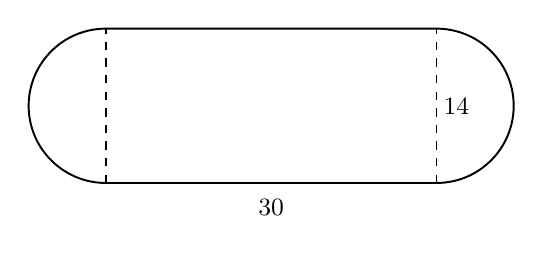
\begin{tikzpicture}[scale=0.14]
\draw[line width=0.7pt] (0,0)--(30,0) arc(-90:90:7)--(0,14) arc(90:270:7)--cycle;
\draw[line width=0.5pt,dashed] (0,0)--(0,14); \draw[line width=0.5pt,dashed] (30,0)--(30,14);
\node[font=\small] at (15,-2.2) {30};
\node[font=\small] at (31.8,7) {14};
\end{tikzpicture}}\par\vspace{2.2mm}
\hspace*{7mm}(A)\ $420+14\pi$\\[1.8mm]
\hspace*{7mm}(B)\ $420+\dfrac{49}{2}\pi$\\[1.8mm]
\hspace*{7mm}(C)\ $420+49\pi$\\[1.8mm]
\hspace*{7mm}(D)\ $420+196\pi$
\vfill}}
\end{textblock*}
\begin{textblock*}{\COLW}(\RCOL,34mm)
{\fontsize{10.4}{13.4}\selectfont
\parbox[t][233mm][t]{\COLW}{%
\noindent\pnum{13} A 20-question quiz awards 5 points for each correct answer and subtracts 2 points for each incorrect answer. Dana answered all 20 questions and needs at least 58 points. What is the least number of questions she must answer correctly?\par\vspace{2.2mm}
\hspace*{7mm}(A)\ $14$\\[1.8mm]
\hspace*{7mm}(B)\ $9$\\[1.8mm]
\hspace*{7mm}(C)\ $12$\\[1.8mm]
\hspace*{7mm}(D)\ $20$
\vfill

\noindent\pnum{14} A museum builds a scale model of the Sun and Earth using one scale for all sizes. In the model, Earth, whose diameter is 12,800 kilometers, is a sphere 4 centimeters in diameter. The Sun's diameter is 1,392,000 kilometers. What is the diameter, in meters, of the model Sun?\gridbox
\vfill

\noindent\pnum{15} Two streaming services opened in the same month. After $t$ months, Service A has $A(t)=800+60t$ thousand subscribers and Service B has $B(t)=500(1.12)^{t}$ thousand subscribers. For the least whole number of months $t$ for which $B(t)>A(t)$, what is the value of $t$?\par\vspace{2.2mm}
\hspace*{7mm}(A)\ $8$\\[1.8mm]
\hspace*{7mm}(B)\ $10$\\[1.8mm]
\hspace*{7mm}(C)\ $13$\\[1.8mm]
\hspace*{7mm}(D)\ $9$
\vfill

\noindent\pnum{16} A candle burns at a constant rate. The graph of its height $h$, in centimeters, $t$ hours after it was lit passes through the points $(2,21)$ and $(6,15)$. Which of the following is the best interpretation of the $t$-intercept of the graph?\par\vspace{2.2mm}
\hspace*{7mm}(A)\ The candle was 24 centimeters tall when it was lit.\\[1.8mm]
\hspace*{7mm}(B)\ The candle burns completely 16 hours after it was lit.\\[1.8mm]
\hspace*{7mm}(C)\ The candle burns 1.5 centimeters every hour.\\[1.8mm]
\hspace*{7mm}(D)\ The candle is 16 centimeters tall after 24 hours.
\vfill}}
\end{textblock*}
\clearpage

% ===== Module 1, page 3 =====
\topicheader{7}{Mock Test 7}
\pagefooter{4}
\colrule{34}{236}
\mbox{}%
\pagekicker{Mock 7 \textperiodcentered{} Module 1 \textperiodcentered{} 22 questions \textperiodcentered{} 35 minutes}{Questions 17--22}
\begin{textblock*}{\COLW}(\LCOL,34mm)
{\fontsize{10.4}{13.4}\selectfont
\parbox[t][233mm][t]{\COLW}{%
\noindent\pnum{17} A cubic polynomial $p$ has a negative leading coefficient. Its graph crosses the $x$-axis at $x=-1$ and touches the $x$-axis at $x=2$ without crossing it. Which of the following could define $p(x)$?\par\vspace{2.2mm}
\hspace*{7mm}(A)\ $-(x+1)^2(x-2)$\\[1.8mm]
\hspace*{7mm}(B)\ $(x+1)(x-2)^2$\\[1.8mm]
\hspace*{7mm}(C)\ $-(x+1)(x-2)^2$\\[1.8mm]
\hspace*{7mm}(D)\ $-(x-1)(x+2)^2$
\vfill

\noindent\pnum{18} A restaurant adds an 8\% sales tax and a 15\% service charge to the food total, both computed on the food total. A party's final bill was \$61.50. What was the food total, in dollars?\gridbox
\vfill

\noindent\pnum{19} Which of the following functions has the greatest maximum value?\par\vspace{2.2mm}
\hspace*{7mm}(A)\ $p(x)=-(x-1)(x+5)$\\[1.8mm]
\hspace*{7mm}(B)\ $q(x)=-3(x-1)^2+4$\\[1.8mm]
\hspace*{7mm}(C)\ $r(x)=-x^2+6x-2$\\[1.8mm]
\hspace*{7mm}(D)\ $s(x)=-\dfrac{1}{2}x^2+2x+6$
\vfill}}
\end{textblock*}
\begin{textblock*}{\COLW}(\RCOL,34mm)
{\fontsize{10.4}{13.4}\selectfont
\parbox[t][233mm][t]{\COLW}{%
\noindent\pnum{20} The quadratic function $f$ has a maximum value of 19. The graph of $y=f(x)$ in the $xy$-plane passes through the points $(1,10)$ and $(7,10)$. What is the value of $f(-1)$?\par\vspace{2.2mm}
\hspace*{7mm}(A)\ $6$\\[1.8mm]
\hspace*{7mm}(B)\ $14$\\[1.8mm]
\hspace*{7mm}(C)\ $44$\\[1.8mm]
\hspace*{7mm}(D)\ $-6$
\vfill

\noindent\pnum{21} A restaurant sells 120 lunch specials per day at a price of $p$ dollars each. When it raises the price by \$1.50, it sells 15 fewer lunch specials per day, and the daily revenue from lunch specials stays exactly the same. What is the daily revenue, in dollars, from lunch specials?\gridbox
\vfill

\noindent\pnum{22} For $0<x<20$, the equation below is true.\dsp{$\sin\left((4x+7)^{\circ}\right)=\cos\left((2x-1)^{\circ}\right)$}What is the value of $x$?\par\vspace{2.2mm}
\hspace*{7mm}(A)\ $29$\\[1.8mm]
\hspace*{7mm}(B)\ $14$\\[1.8mm]
\hspace*{7mm}(C)\ $41$\\[1.8mm]
\hspace*{7mm}(D)\ $84$
\vfill}}
\end{textblock*}
\clearpage

% ===== Module 2, page 1 =====
\topicheader{7}{Mock Test 7}
\pagefooter{5}
\colrule{34}{236}
\mbox{}%
\pagekicker{Mock 7 \textperiodcentered{} Module 2 \textperiodcentered{} 22 questions \textperiodcentered{} 35 minutes}{Questions 1--8}
\begin{textblock*}{\COLW}(\LCOL,34mm)
{\fontsize{10.4}{13.4}\selectfont
\parbox[t][233mm][t]{\COLW}{%
\noindent\pnum{1} If $5-2x=3x-15$, what is the value of $x$?\par\vspace{2.2mm}
\hspace*{7mm}(A)\ $-10$\\[1.8mm]
\hspace*{7mm}(B)\ $4$\\[1.8mm]
\hspace*{7mm}(C)\ $-2$\\[1.8mm]
\hspace*{7mm}(D)\ $20$
\vfill

\noindent\pnum{2} The function $f$ is defined by $f(x)=x^2-3x+5$. What is the value of $f(-2)$?\par\vspace{2.2mm}
\hspace*{7mm}(A)\ $3$\\[1.8mm]
\hspace*{7mm}(B)\ $7$\\[1.8mm]
\hspace*{7mm}(C)\ $-5$\\[1.8mm]
\hspace*{7mm}(D)\ $15$
\vfill

\noindent\pnum{3} On an excavation plan, 1 centimeter represents 0.5 meter. A rectangular trench appears on the plan as 6 centimeters by 4.5 centimeters. What is the actual area, in square meters, of the trench?\par\vspace{2.2mm}
\hspace*{7mm}(A)\ $6.75$\\[1.8mm]
\hspace*{7mm}(B)\ $10.5$\\[1.8mm]
\hspace*{7mm}(C)\ $13.5$\\[1.8mm]
\hspace*{7mm}(D)\ $27$
\vfill

\noindent\pnum{4} The graph of $5x+ky=20$ in the $xy$-plane, where $k$ is a constant, passes through the point $(2,5)$. What is the $y$-coordinate of the $y$-intercept of the graph?\gridbox
\vfill}}
\end{textblock*}
\begin{textblock*}{\COLW}(\RCOL,34mm)
{\fontsize{10.4}{13.4}\selectfont
\parbox[t][233mm][t]{\COLW}{%
\noindent\pnum{5} The graph of the quadratic function $f$ in the $xy$-plane opens upward, has its vertex at $(3,-4)$, and passes through the point $(5,4)$. Which of the following defines $f$?\par\vspace{2.2mm}
\hspace*{7mm}(A)\ $2(x+3)^2-4$\\[1.8mm]
\hspace*{7mm}(B)\ $4(x-3)^2-4$\\[1.8mm]
\hspace*{7mm}(C)\ $2(x-3)^2-4$\\[1.8mm]
\hspace*{7mm}(D)\ $2(x-3)^2+4$
\vfill

\noindent\pnum{6} Triangles $X$, $Y$, and $Z$ are similar. Every side of $Y$ is 3 times as long as the corresponding side of $X$, and every side of $Z$ is $\frac{2}{3}$ as long as the corresponding side of $Y$. The area of triangle $Z$ is 100 square units. What is the area of triangle $X$?\par\vspace{2.2mm}
\hspace*{7mm}(A)\ $50$\\[1.8mm]
\hspace*{7mm}(B)\ $200$\\[1.8mm]
\hspace*{7mm}(C)\ $400$\\[1.8mm]
\hspace*{7mm}(D)\ $25$
\vfill

\noindent\pnum{7} If $3x+5y=17$ and $2x-y=7$, what is the value of $5x+4y$?\par\vspace{2.2mm}
\hspace*{7mm}(A)\ $24$\\[1.8mm]
\hspace*{7mm}(B)\ $7$\\[1.8mm]
\hspace*{7mm}(C)\ $10$\\[1.8mm]
\hspace*{7mm}(D)\ $17$
\vfill

\noindent\pnum{8} The function $f$ is defined by $f(x)=a\cdot b^{x}$, where $a$ and $b$ are positive constants. If $f(1)=12$ and $f(3)=48$, what is the value of $f(0)$?\gridbox
\vfill}}
\end{textblock*}
\clearpage

% ===== Module 2, page 2 =====
\topicheader{7}{Mock Test 7}
\pagefooter{6}
\colrule{34}{236}
\mbox{}%
\pagekicker{Mock 7 \textperiodcentered{} Module 2 \textperiodcentered{} 22 questions \textperiodcentered{} 35 minutes}{Questions 9--15}
\begin{textblock*}{\COLW}(\LCOL,34mm)
{\fontsize{10.4}{13.4}\selectfont
\parbox[t][233mm][t]{\COLW}{%
\noindent\pnum{9} The table shows two data sets, $P$ and $Q$, each with six values. Which of the following statements is true?\figwrap{\begin{tabular}{|l|c|c|c|c|c|c|}
\hline
Set $P$ & 8 & 8 & 8 & 14 & 14 & 14\\\hline
Set $Q$ & 8 & 9 & 10 & 12 & 13 & 14\\\hline
\end{tabular}}\par\vspace{2.2mm}
\hspace*{7mm}(A)\ The two sets have the same mean and the same median, and Set $Q$ has the greater standard deviation.\\[1.8mm]
\hspace*{7mm}(B)\ The two sets have the same mean and the same median, and Set $P$ has the greater standard deviation.\\[1.8mm]
\hspace*{7mm}(C)\ The two sets have the same mean, but Set $P$ has the greater median.\\[1.8mm]
\hspace*{7mm}(D)\ The two sets have the same median, but Set $Q$ has the greater mean.
\vfill

\noindent\pnum{10} A glass supplier accepts a pane if its thickness $t$, in millimeters, satisfies $|t-6.4|\le0.15$. What is the difference, in millimeters, between the greatest and the least acceptable thickness?\par\vspace{2.2mm}
\hspace*{7mm}(A)\ $0.15$\\[1.8mm]
\hspace*{7mm}(B)\ $6.25$\\[1.8mm]
\hspace*{7mm}(C)\ $0.30$\\[1.8mm]
\hspace*{7mm}(D)\ $6.55$
\vfill

\noindent\pnum{11} For all values of $x$, $(x+3)(x^2-2x+k)=x^3+x^2-2x+c$, where $k$ and $c$ are constants. What is the value of $c$?\gridbox
\vfill

\noindent\pnum{12} A survey drone's height above an archaeological site, in meters, $t$ minutes after launch is $h=40+12t$. What is the height of the drone, in meters, 150 seconds after launch?\par\vspace{2.2mm}
\hspace*{7mm}(A)\ $58$\\[1.8mm]
\hspace*{7mm}(B)\ $70$\\[1.8mm]
\hspace*{7mm}(C)\ $190$\\[1.8mm]
\hspace*{7mm}(D)\ $1{,}840$
\vfill}}
\end{textblock*}
\begin{textblock*}{\COLW}(\RCOL,34mm)
{\fontsize{10.4}{13.4}\selectfont
\parbox[t][233mm][t]{\COLW}{%
\noindent\pnum{13} Kepler's third law states that for planets orbiting the same star, the square of a planet's orbital period is proportional to the cube of its average distance from the star. Planet $Y$ has an orbital period 8 times that of Planet $X$. Assume both planets move in circular orbits at constant speeds. Planet $Y$'s orbital speed is how many times Planet $X$'s orbital speed?\par\vspace{2.2mm}
\hspace*{7mm}(A)\ $\dfrac{1}{2}$\\[1.8mm]
\hspace*{7mm}(B)\ $\dfrac{1}{8}$\\[1.8mm]
\hspace*{7mm}(C)\ $2$\\[1.8mm]
\hspace*{7mm}(D)\ $4$
\vfill

\noindent\pnum{14} An archaeologist counted the pottery fragments in each of five trenches. Each count is a positive integer, the mean of the five counts is 14, and the median is 12. What is the greatest possible number of fragments in the trench with the most fragments?\gridbox
\vfill

\noindent\pnum{15} For how many integer values of $k$ does the equation $(k-3)x=12$ have an integer solution $x$?\par\vspace{2.2mm}
\hspace*{7mm}(A)\ $6$\\[1.8mm]
\hspace*{7mm}(B)\ $11$\\[1.8mm]
\hspace*{7mm}(C)\ $13$\\[1.8mm]
\hspace*{7mm}(D)\ $12$
\vfill}}
\end{textblock*}
\clearpage

% ===== Module 2, page 3 =====
\topicheader{7}{Mock Test 7}
\pagefooter{7}
\colrule{34}{236}
\mbox{}%
\pagekicker{Mock 7 \textperiodcentered{} Module 2 \textperiodcentered{} 22 questions \textperiodcentered{} 35 minutes}{Questions 16--22}
\begin{textblock*}{\COLW}(\LCOL,34mm)
{\fontsize{10.4}{13.4}\selectfont
\parbox[t][233mm][t]{\COLW}{%
\noindent\pnum{16} The table gives four values of the quadratic function $f$. The function $g$ is defined by $g(x)=f(2x-1)+8$. What is the greatest value of $x$ for which $g(x)=0$?\figwrap{\begin{tabular}{|c|c|c|c|c|}
\hline
$x$ & 0 & 1 & 3 & 5\\\hline
$f(x)$ & $-5$ & $-8$ & $-8$ & 0\\\hline
\end{tabular}}\par\vspace{2.2mm}
\hspace*{7mm}(A)\ $1$\\[1.8mm]
\hspace*{7mm}(B)\ $3$\\[1.8mm]
\hspace*{7mm}(C)\ $2$\\[1.8mm]
\hspace*{7mm}(D)\ $7$
\vfill

\noindent\pnum{17} In the $xy$-plane, the circle with equation $x^2+y^2-4x+6y-212=0$ and the point $P(26,4)$ are given. The two lines through $P$ that are tangent to the circle touch it at points $T_1$ and $T_2$. What is the length of $\overline{T_1T_2}$?\par\vspace{2.2mm}
\hspace*{7mm}(A)\ $12$\\[1.8mm]
\hspace*{7mm}(B)\ $24$\\[1.8mm]
\hspace*{7mm}(C)\ $20$\\[1.8mm]
\hspace*{7mm}(D)\ $30$
\vfill

\noindent\pnum{18} What is the sum of all real solutions of the equation $x^{2/3}-5x^{1/3}+6=0$?\gridbox
\vfill

\noindent\pnum{19} Two cell towers are located at mile markers 4 and 10 along a straight highway. A driver at mile marker $x$ has a combined distance to the two towers that is less than 10 miles. For how many integer values of $x$ is this possible?\par\vspace{2.2mm}
\hspace*{7mm}(A)\ $7$\\[1.8mm]
\hspace*{7mm}(B)\ $11$\\[1.8mm]
\hspace*{7mm}(C)\ $13$\\[1.8mm]
\hspace*{7mm}(D)\ $9$
\vfill}}
\end{textblock*}
\begin{textblock*}{\COLW}(\RCOL,34mm)
{\fontsize{10.4}{13.4}\selectfont
\parbox[t][233mm][t]{\COLW}{%
\noindent\pnum{20} In the $xy$-plane, lines $\ell$ and $n$ are perpendicular and intersect at the point $(2,5)$. The $y$-intercept of $n$ is 5 greater than the $y$-intercept of $\ell$. If the slope of $\ell$ is positive and greater than 1, what is the slope of $\ell$?\par\vspace{2.2mm}
\hspace*{7mm}(A)\ $-\dfrac{1}{2}$\\[1.8mm]
\hspace*{7mm}(B)\ $\dfrac{1}{2}$\\[1.8mm]
\hspace*{7mm}(C)\ $2$\\[1.8mm]
\hspace*{7mm}(D)\ $5$
\vfill

\noindent\pnum{21} In the figure, triangle $ABC$ has a right angle at $C$, with $CA=8$ and $CB=6$. Semicircles are drawn outward on legs $\overline{CA}$ and $\overline{CB}$, and the circle with diameter $\overline{AB}$ is drawn through $C$. The two shaded crescents lie inside the semicircles but outside the large circle. What is the total area of the two shaded regions?\figwrap{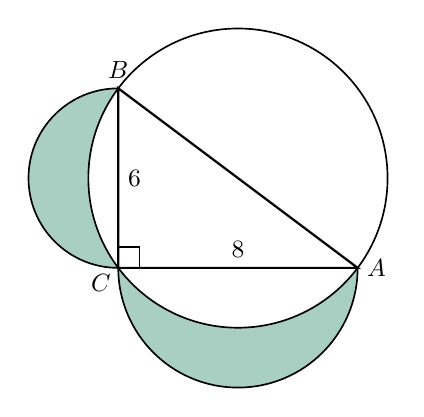
\begin{tikzpicture}[scale=0.38]
\coordinate (C) at (0,0); \coordinate (A) at (8,0); \coordinate (B) at (0,6);
\fill[badge] (0,0) arc(180:360:4)--cycle;
\fill[badge] (0,6) arc(90:270:3)--cycle;
\fill[white] (4,3) circle (5);
\draw[line width=0.6pt] (0,0) arc(180:360:4);
\draw[line width=0.6pt] (0,6) arc(90:270:3);
\draw[line width=0.6pt] (4,3) circle (5);
\draw[line width=0.8pt] (C)--(A)--(B)--cycle;
\draw[line width=0.5pt] (0,0.7)--(0.7,0.7)--(0.7,0);
\node[font=\small] at (-0.6,-0.5) {$C$}; \node[right,font=\small] at (A) {$A$}; \node[above,font=\small] at (B) {$B$};
\node[above,font=\small] at (4,0) {8}; \node[right,font=\small] at (0,3) {6};
\end{tikzpicture}}\gridbox
\vfill

\noindent\pnum{22} For how many integer values of $p$ does the equation $x^2-px+24=0$ have two integer solutions?\par\vspace{2.2mm}
\hspace*{7mm}(A)\ $8$\\[1.8mm]
\hspace*{7mm}(B)\ $4$\\[1.8mm]
\hspace*{7mm}(C)\ $16$\\[1.8mm]
\hspace*{7mm}(D)\ $12$
\vfill}}
\end{textblock*}
\clearpage

\end{document}
